%This is the homework 2 latex file for problem 2

\documentclass{article}
\usepackage{amsfonts}
\usepackage{amssymb}
\usepackage{graphicx}
\usepackage{mathtools}
\usepackage{color}
\usepackage{fancyhdr}
\usepackage[margin=2cm]{geometry}
\DeclarePairedDelimiter\ceil{\lceil}{\rceil}
\DeclarePairedDelimiter\floor{\lfloor}{\rfloor}
\pagestyle{fancy}


\begin{document}
\fancyhfoffset[L]{0cm}
\fancyhfoffset[R]{0cm}
\chead{Tyler Ayrton Stank}

\begin{enumerate}
    \setcounter{enumi}{1}
    %2
    \item
    \begin{enumerate}
        %2a
        \item
            The second and fifth members are correctly classified, while the first, third, and fourth fail.  The test accuracy is $\frac{2}{5} = 0.4$.

        %2b
        \item \textcolor{white}{.}\vspace{-1em}\\
            \begin{tabular}{|c|c|c|}\hline
                \textbf{Node pruned} & \textbf{Classifier raplacement} & \textbf{Classification accuracy} \\\hline
                $A \ge 1.5$ & C2 & 0.8 \\\hline
                    % pass pass fail pass pass
                $B \ge 1.7$ & C1 & 0.4 \\\hline
                    % fail pass fail fail pass
                $A \ge 1.7$ & C2 & 0.6 \\\hline
                    % pass pass fail pass fail
                $A \ge 0.6$ & C1 & 0.6 \\\hline
                    % fail pass pass fail pass
            \end{tabular}\\\textcolor{white}{.}\vspace{1em}\\
            \begin{tabular}{p{6cm} p{6cm}}
                $A \ge 1.5$ pruned & $B \ge 1.7$ pruned \\
                %\includegraphics[width=5cm,raise=-1em]{P2bi}   & \includegraphics[width=5cm]{P2bii} \\\textcolor{white}{.}\\ %Don't need vspace, as this creates a row in the table
                \raisebox{-\height}{\includegraphics[width=5cm]{P2bi}}     & \raisebox{-\height}{\includegraphics[width=5cm]{P2bii}}\\
                $A \ge 1.7$ pruned & $A \ge 0.6$ pruned \\
                %\includegraphics[width=5cm]{P2biii} & \includegraphics[width=5cm]{P2biv}
                \raisebox{-\height}{\includegraphics[width=5cm]{P2biii}}   & \raisebox{-\height}{\includegraphics[width=5cm]{P2biv}}\\
            \end{tabular}
                % 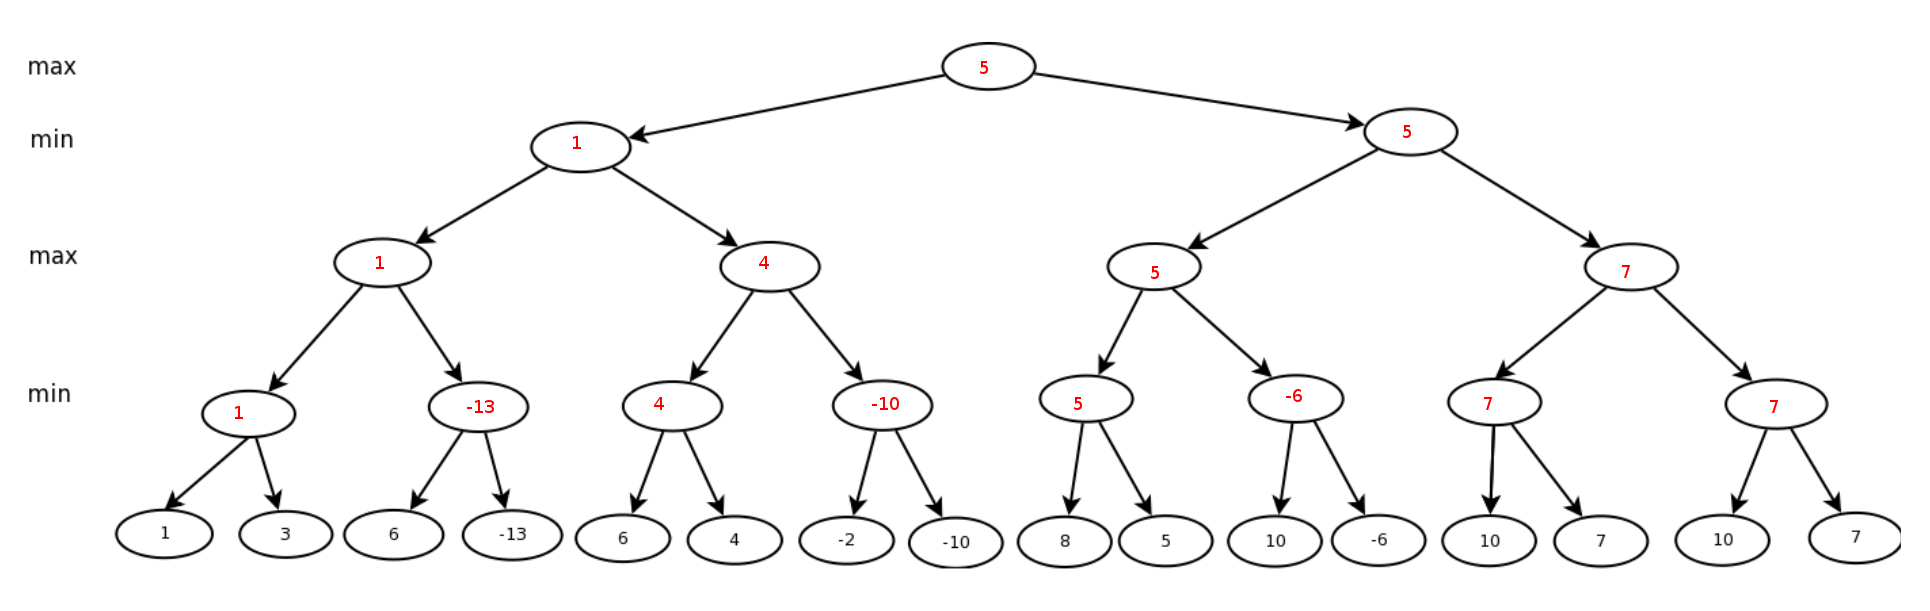
\includegraphics[width=0.9\textwidth]{P1a}

        %2c
        \item
            The last question node (which asks $A\ge 1.5$?) should be pruned--the accuracy on the tune set with this pruning is 0.8.\\
            \includegraphics[width=6cm]{P2bi}

    \end{enumerate}
\end{enumerate}

\end{document}


%
%   Test 1 fail
%   Test 2 pass
%   Test 3 fail
%   Test 4 fail
%   Test 5 pass
%
%
%
